\subsection{Mikrocontroller}\label{subsec:Hardware_Mikrocontroller}
Der Test des Mikrocontrollers soll eine reine Funktionskontrolle mit Überprüfung der Datenübertragung sein, welche das Zusammenspiel zwischen Display, Mikrocontroller, Pumpen und Motorentreiber testet. 

\subsubsection{Systemtest}\label{subsubsec:Hardware_Systemtest}

Der Test sieht wie folgt aus:

\begin{enumerate}
\item Bei Druck auf den Button des Displays:
\begin{itemize}
\item Button-ID wird vom Display an den Mikrocontroller gesendet.
\item Mikrocontroller verarbeitet die ID.
\\
\end{itemize}
\item Bei der ID (0xFF 0xB1 0xFF 0xFF 0xFF) löst der Mikrocontroller folgende Testfunktionen aus:
\begin{itemize}
\item Mikrocontroller initialisiert den TMC4671.
\item Mikrocontroller ändert Text und Bild auf Display.
\item Mikrocontroller toggelt eine LED (Simuliert die Ansteuerung eines FET)
\end{itemize}
\end{enumerate}

\subsubsection{Erwartung}\label{subsubsec:Hardware_Gesamtsystem_Erwartung}

Wird der Menu-Button 0xB1 auf der Seite 0xFF gedrückt, so wird erwartet, dass der Mikrocontroller die Funktionen in folgender Reihenfolge abarbeitet. 
\begin{enumerate}
\item Statusübermittlung
\begin{itemize}
\item UART\_0-Schnittstelle muss angesprochen werden.
\item Vor jedem Ausführen einer Funktion teilt der Mikrocontroller dem Computer mit, an welchem Punkt der Software er sich gerade befindet.
\end{itemize}
\item Initialisierung TMC
\begin{itemize}
\item SPI-Schnittstelle muss angesprochen werden.
\item Motor dreht sich noch nicht.
\end{itemize}
\item Text und Bild ändern
\begin{itemize}
\item UART\_1-Schnittstelle muss angesprochen werden.
\item Gin-Tonic-Text muss mit Lemon Soda ersetzt werden.
\item Bild von Gin-Tonic muss mit anderem Bild ersetzt werden.
\end{itemize}
\item LED-Toggeln (Simuliert die Ansteuerung eines FET)
\begin{itemize}
\item Die Hardware des Mikrocontrollers muss angesprochen werden
%(im Programmfluss Änderung eines Status).
\item LED toggelt bei jeder Beführung des Buttons.
\end{itemize}

\end{enumerate}

%Für die Initialisierung des TMC wird die SPI-Schnittstelle muss die SPI-Schnittstelle angesprochen werden. für die Änderung des Text- und Bildes muss die UART\_1-Schnittstelle angesprochen werden, die LED muss die Hardware des Mikrocontrollers an 

%\paragraph{Display}\mbox{}\\

%Die Funktion des Displays wurde bereits in Kapitel \ref{subsubsec:Display_Test} getestet und bedarf keiner weiteren Tests in der Funktionsprüfung.

%\paragraph{Mikrocontroller}\mbox{}\\

%\subparagraph{Erkennen und Interpretieren der einkommenden Daten des Displays.}\mbox{}\\

%Je nach dem, ob der Button 0xB1 der Seite 0xFF oder ob der Button 0x01 der Seite 0x07 gedrückt wurden, werden verschiedene Funktionsabläufe aufgerufen.

%Mit dem Button 0xB1 auf der Seite 0xFF werden die Testfunktionen aufgerufen, mit dem Button 0x01 auf der Seite 0x07 wird ein Ablauf gestartet, welcher eher einem Ablauf in der Realität entspricht.

%\subparagraph{Ausgabe aller Vorgänge im Mikrocontroller.}\mbox{}\\
%Schreiben UART\_0

\subsubsection{Ergebnis}\label{subsubsec:Hardware_Gesamtsystem_Ergebnis}

Folgende Ergebnisse wurden beim Test erzielt:
\begin{enumerate}
\item Statusübermittlung\\
\\
Wie in Abbildung \ref{fig:Hardware_Uart_0_0} zu sehen ist, funktioniert die Übertragung einwandfrei. Der Mikrocontroller läuft durch die Software und zeigt, an welcher Stelle er ist. Die Funktion ist somit bestätigt.

\begin{figure}[h!]
	\centering	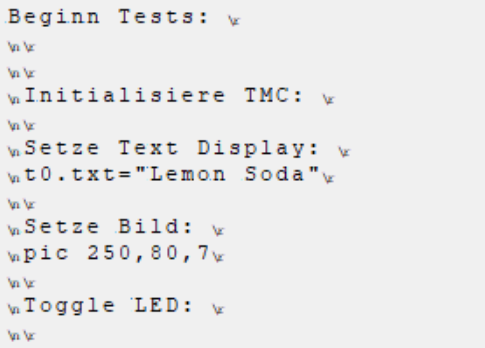
\includegraphics[width=0.5\textwidth]{graphics/Test_UART0_0.png}
	\caption{Ausgabe der abzuhandelnden Schritte, wie sie gemäss Button 0xB1 der Seite 0xFF programmiert wurden, an die USB-Schnittstelle.} 
	\label{fig:Hardware_Uart_0_0}
\end{figure}

\newpage

\item Initialisierung TMC\\
\\
In Abbildung \ref{fig:Hardware_SPI_TMC4671_Beginn} ist zu erkennen, dass die Übertragung korrekt ausgegeben wird. Da die gesamte Übertragung zu gross ist, wurde das Ende dokumentiert, erkennbar in der Abbildung \ref{fig:Hardware_SPI_TMC4671_Ende}. Die Initialisierung konnte so nicht dokumentiert werden aufgrund der Probleme mit dem EVAL-Board. Die Initialisierung gilt deshalb noch als teilverifiziert. Die komplette Implementierung des Chips wird Teil des Projekt 6 sein.

\begin{figure}[h!]
	\centering	
	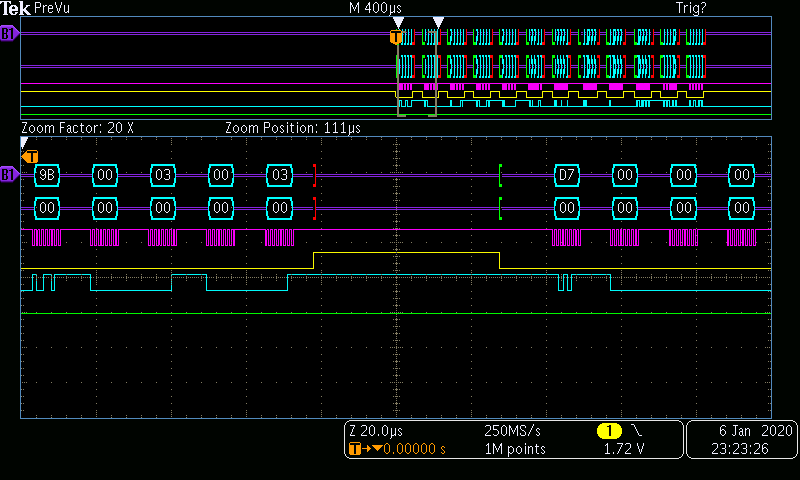
\includegraphics[width=0.8\textwidth]{graphics/TEST_Beginn_TMC_Initialisierung.png}
	\caption{Beginn der Ausgabe der SPI-Schnittstelle, wie sie gemäss TMC4671\_init() programmiert wurde.} 
	\label{fig:Hardware_SPI_TMC4671_Beginn}
\end{figure}
\begin{figure}[h!]
	\centering	
	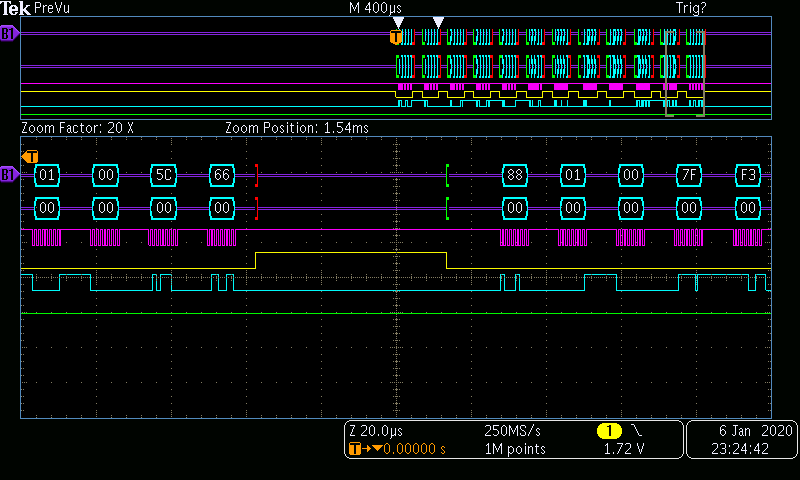
\includegraphics[width=0.8\textwidth]{graphics/TEST_Ende_TMC_Initialisierung.png}
	\caption{Ende der Ausgabe der SPI-Schnittstelle, wie sie gemäss TMC4671\_init() programmiert wurde.} 
	\label{fig:Hardware_SPI_TMC4671_Ende}
\end{figure}

\newpage
\item Text und Bild ändern\\
\\

Abbildung \ref{fig:Hardware_Text_Bild_vor_Button} zeigt den ersten Bildschirm, wenn es eingeschaltet wird. Nachdem der Button ``Menue`` gedrückt wurde, wird der Text von Gin Tonic zu Lemon Soda geändert und das Bild mit dem Drink wird gewechselt. Die Funktion gilt als bestätigt.

\begin{figure}[h!]
\centering
\subcaptionbox{Seite 0xFF bevor der Button gedrückt wird.\label{fig:Hardware_Text_Bild_vor_Button}}{	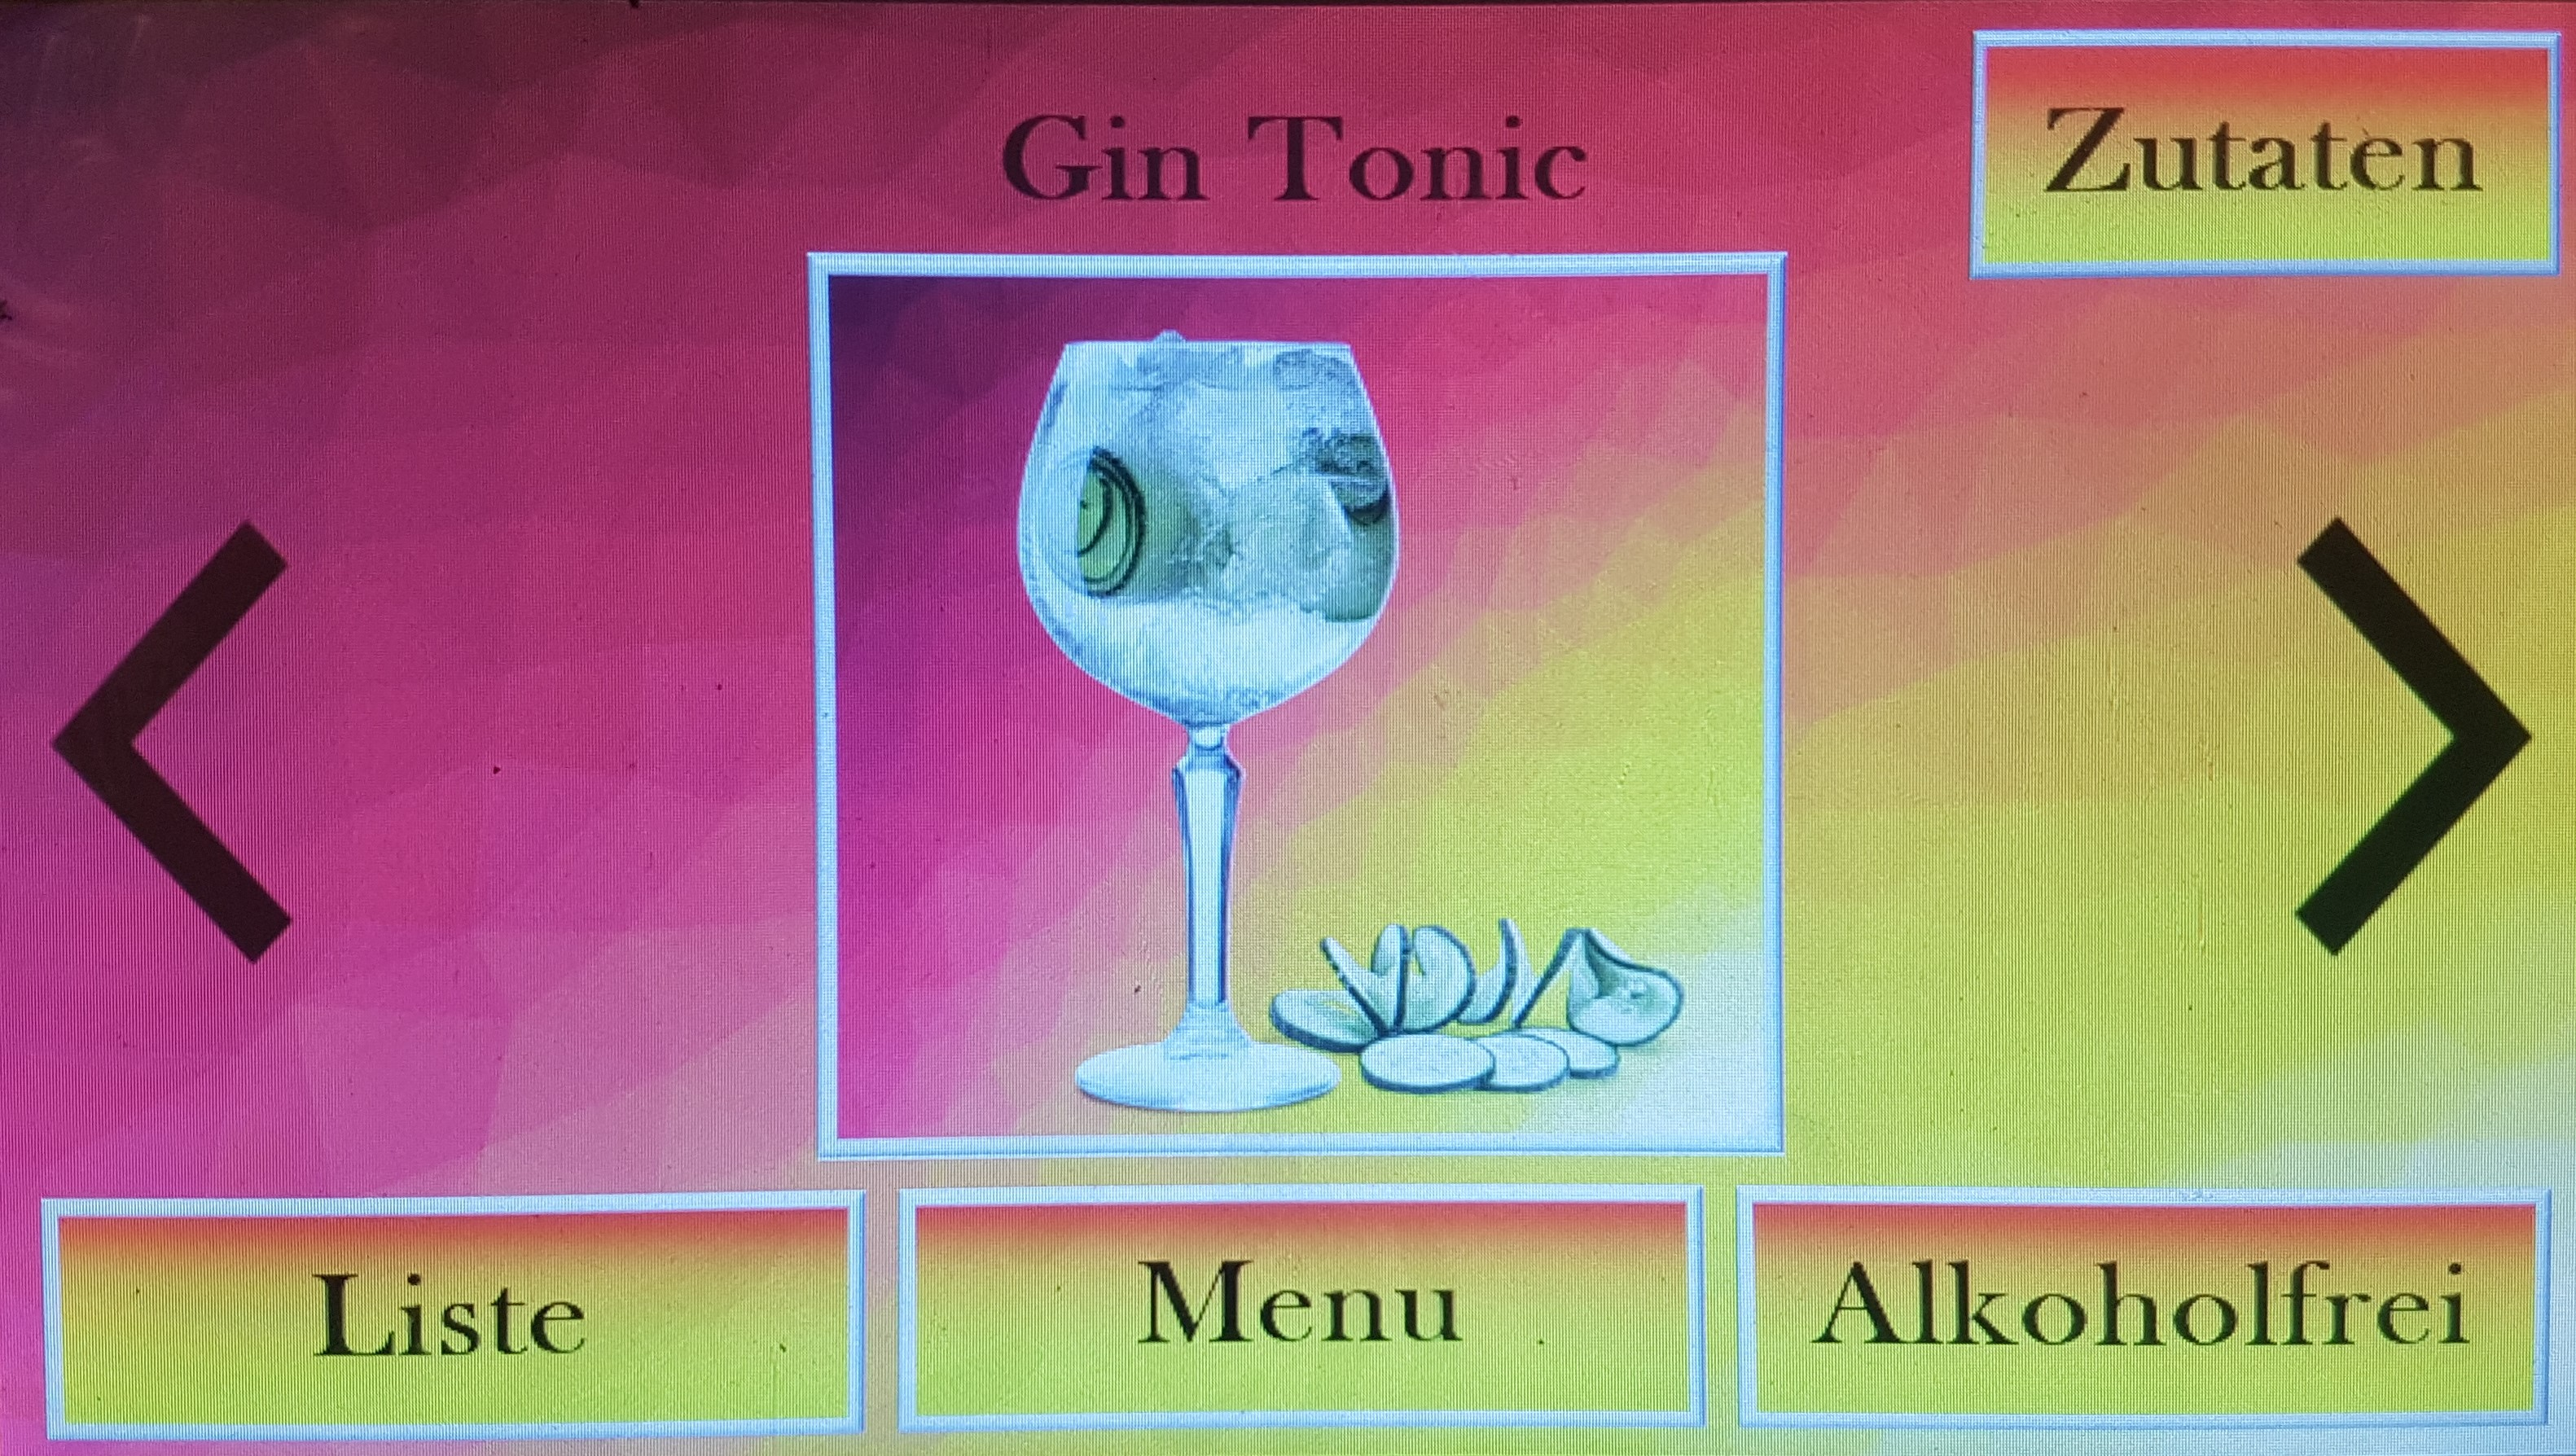
\includegraphics[width=0.48\textwidth]{graphics/Display_Gin_Tonic_Startseite.jpg}}
\hfill
\subcaptionbox{Seite 0xFF nachdem der Button gedrückt wird.\label{fig:Hardware_Text_Bild_nach_Button}}{	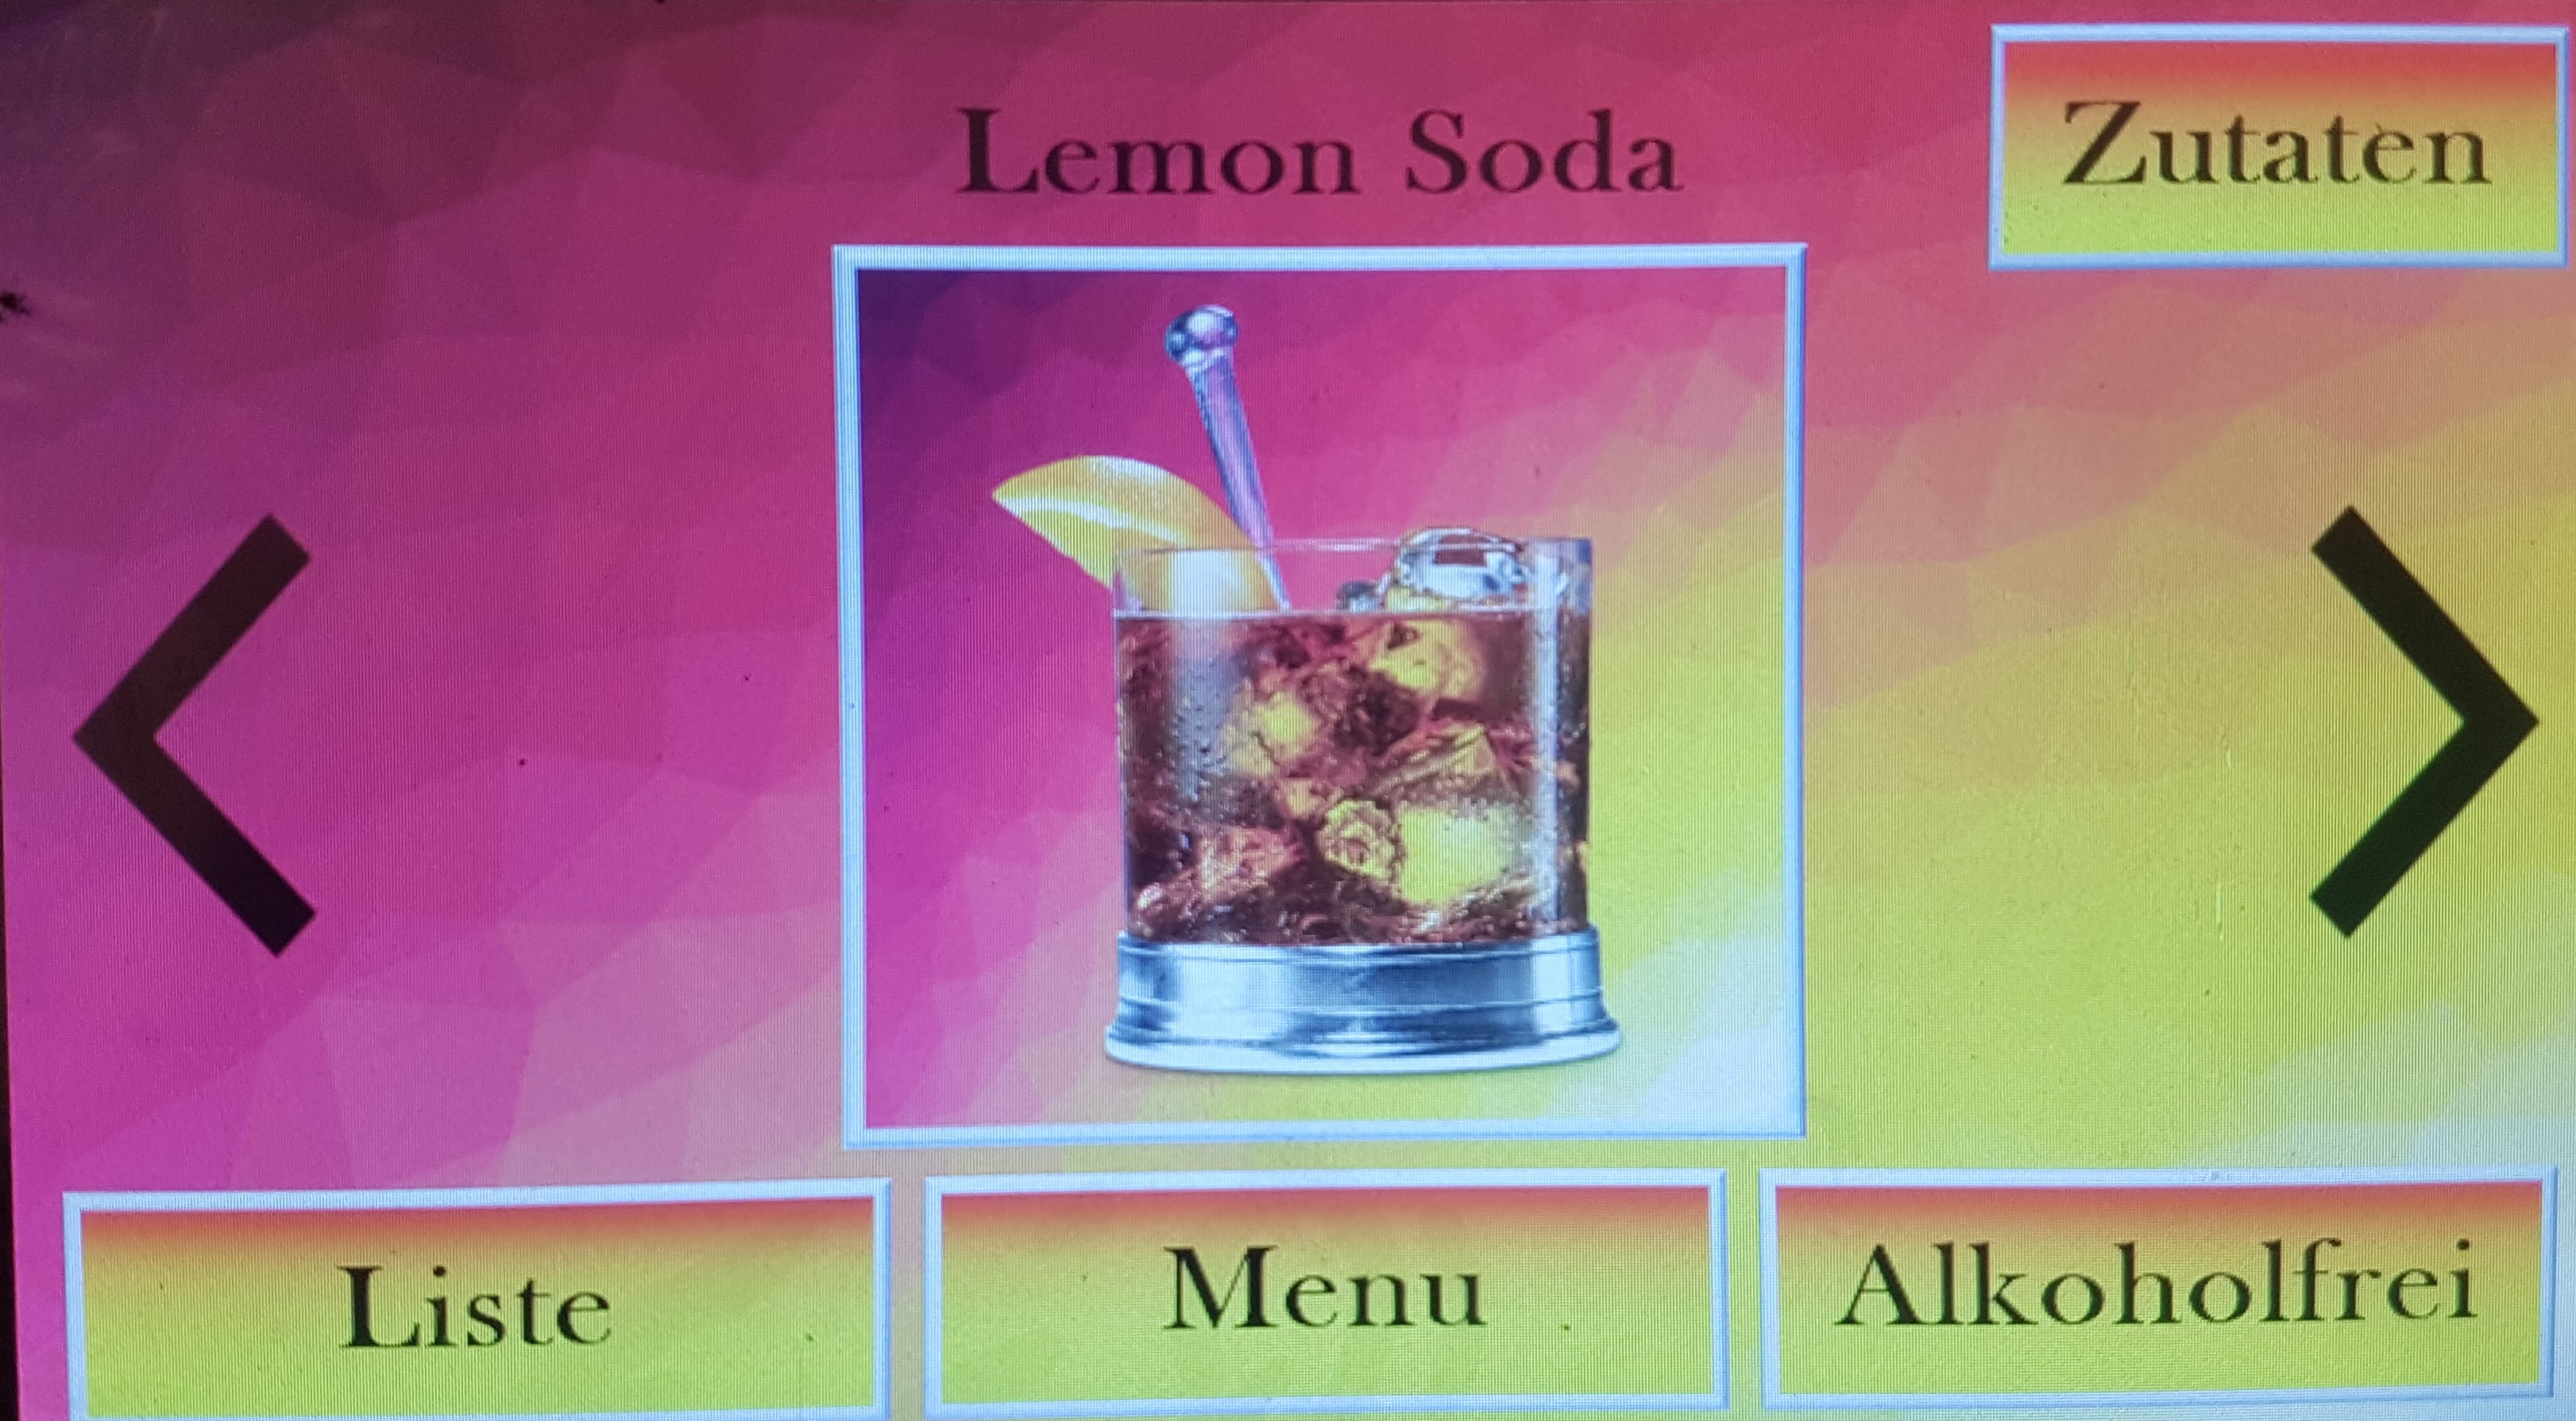
\includegraphics[width=0.48\textwidth]{graphics/Display_Lemon_Soda_Startseite.jpg}}
\hfill
\caption{Bildschirmanzeigen vor und nach dem Drücken des Buttons.}
\label{fig:Hardware_Text_Bild}
\end{figure}
\newpage

\item LED toggeln\\
\\
Wie in Abbildung \ref{fig:Hardware_LED_FET_eingeschalten} ersichtlich, geht die eingebaute LED des Arduino-Mega-Boards an. Sobald erneut auf den Button gedrückt wird, geht diese wieder aus wie in Abbildung \ref{fig:Hardware_LED_FET_ausgeschalten} erkennbar ist. Die Ansteuerung eines FET während des Programmflusses ist somit verifiziert.

\begin{figure}[h!]
\centering
\subcaptionbox{Von Mikrocontroller eingeschaltene LED.\label{fig:Hardware_LED_FET_eingeschalten}}{	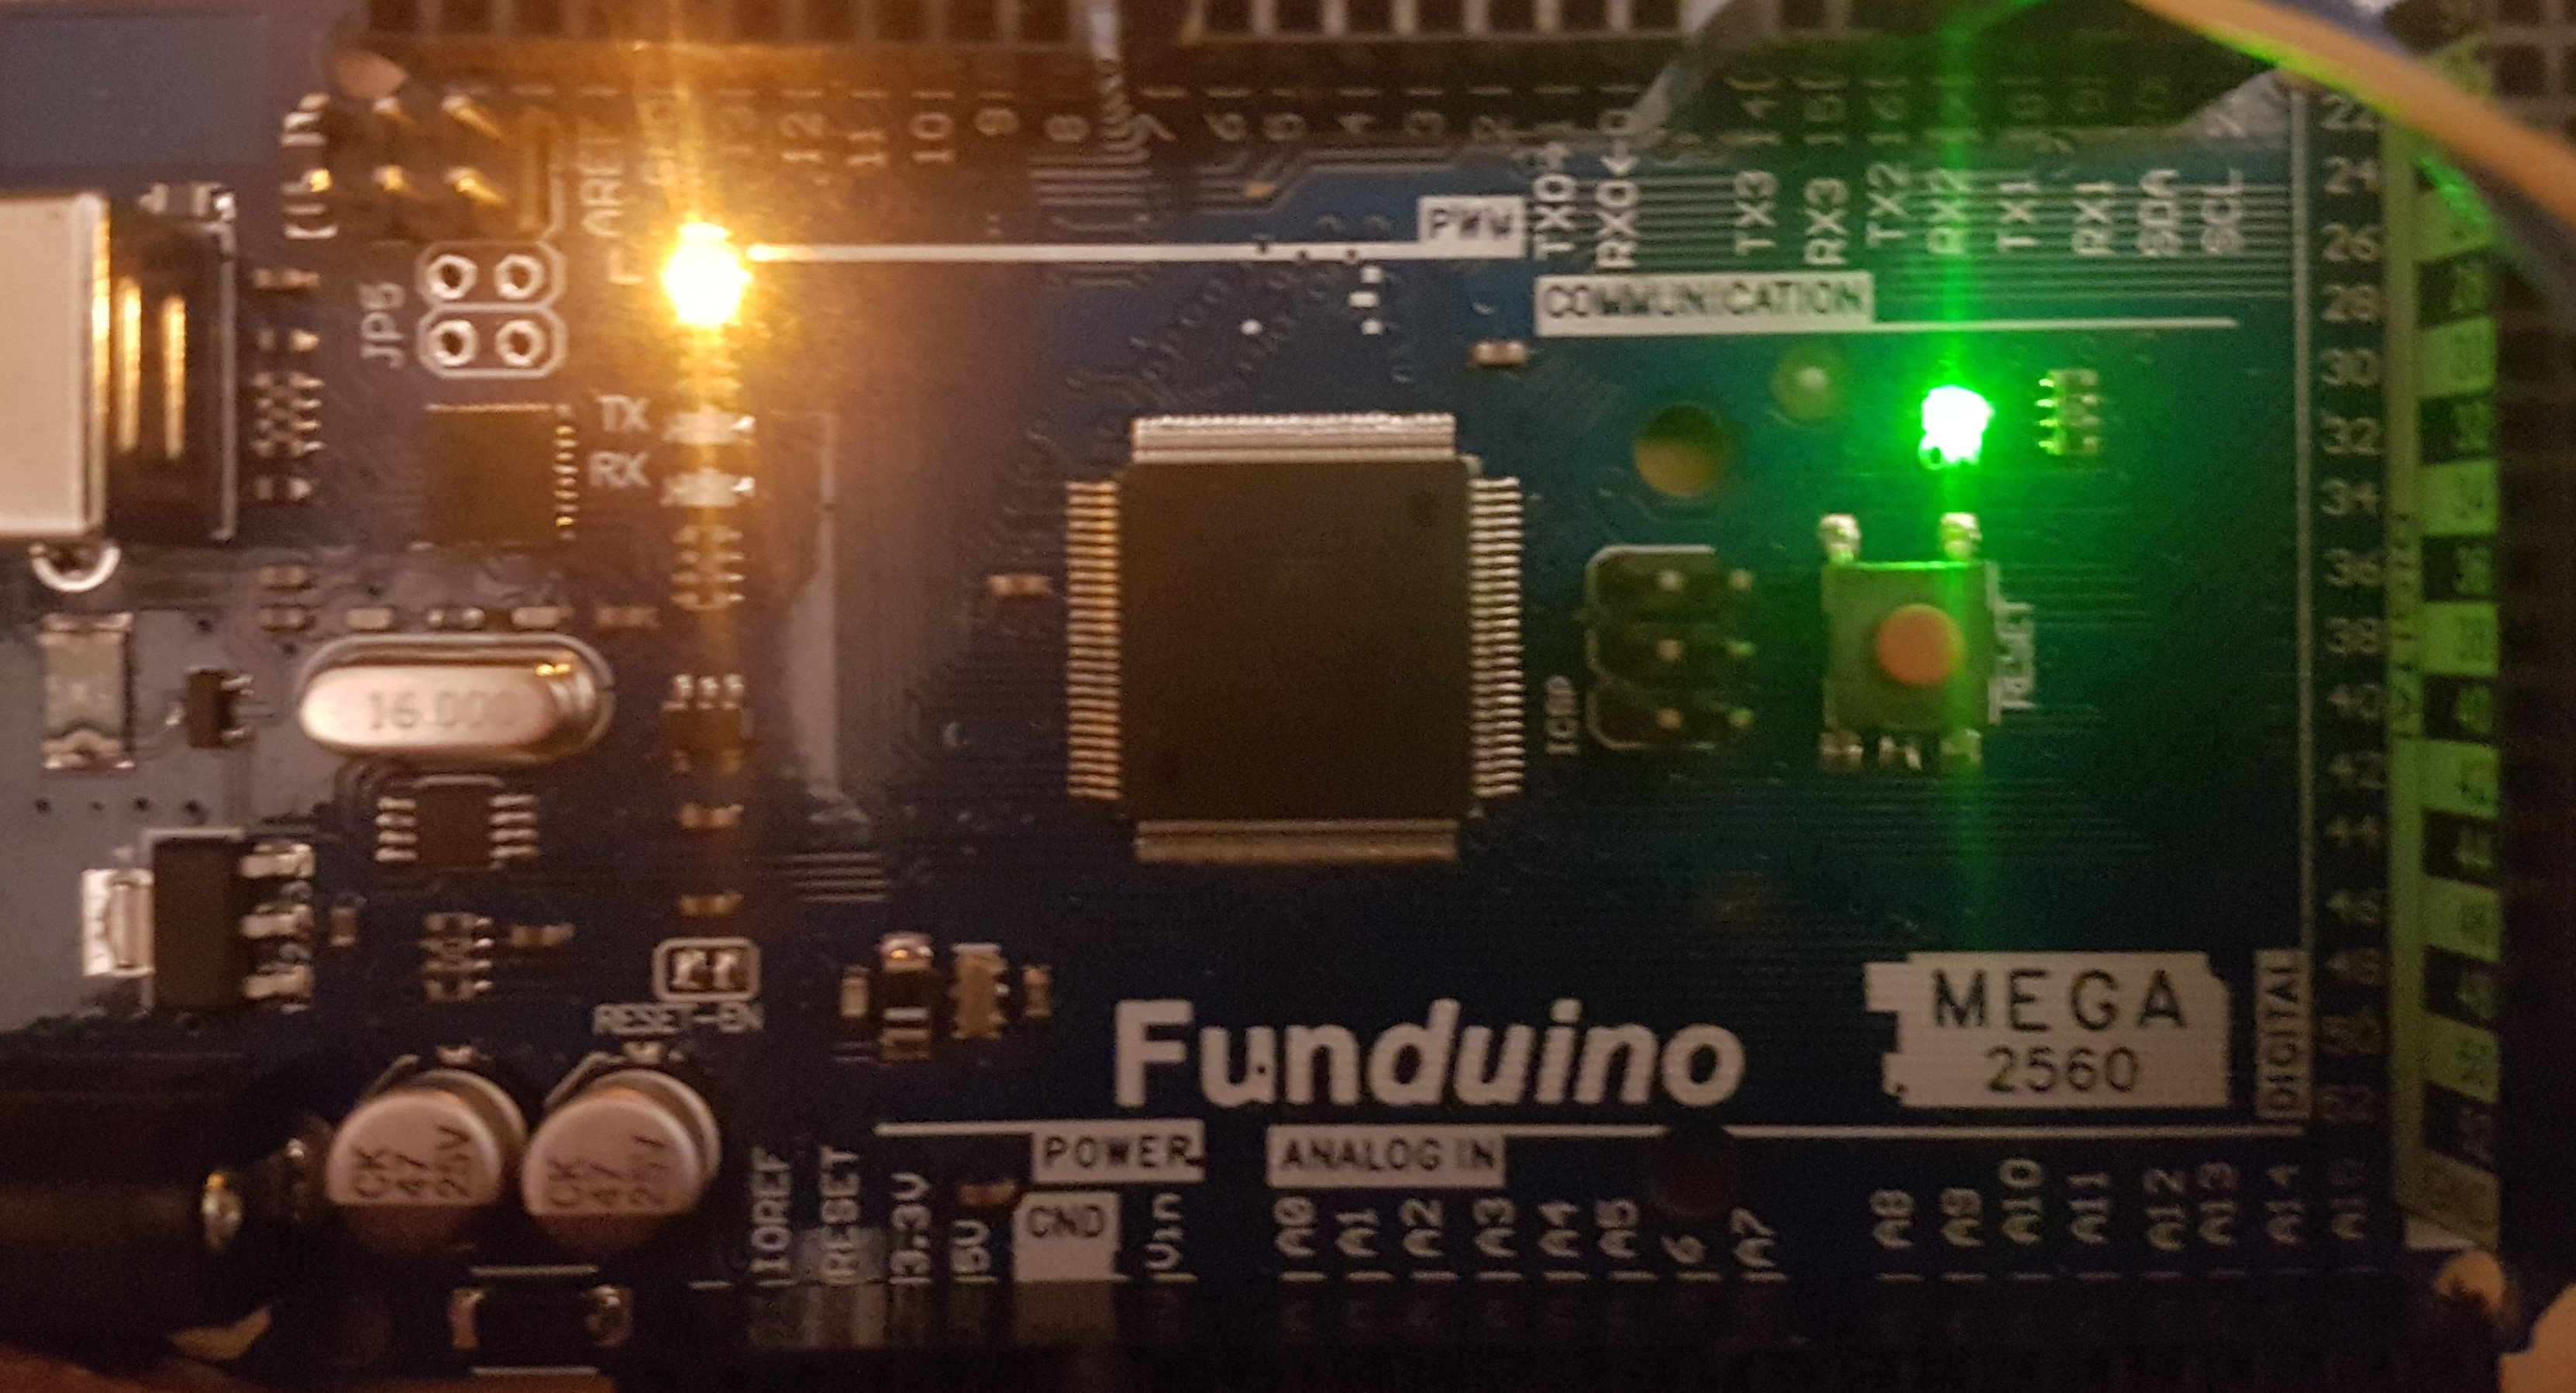
\includegraphics[width=0.48\textwidth]{graphics/Display_LED_ON.jpg}}
\hfill
\subcaptionbox{Von Mikrocontroller ausgeschaltene LED.\label{fig:Hardware_LED_FET_ausgeschalten}}{	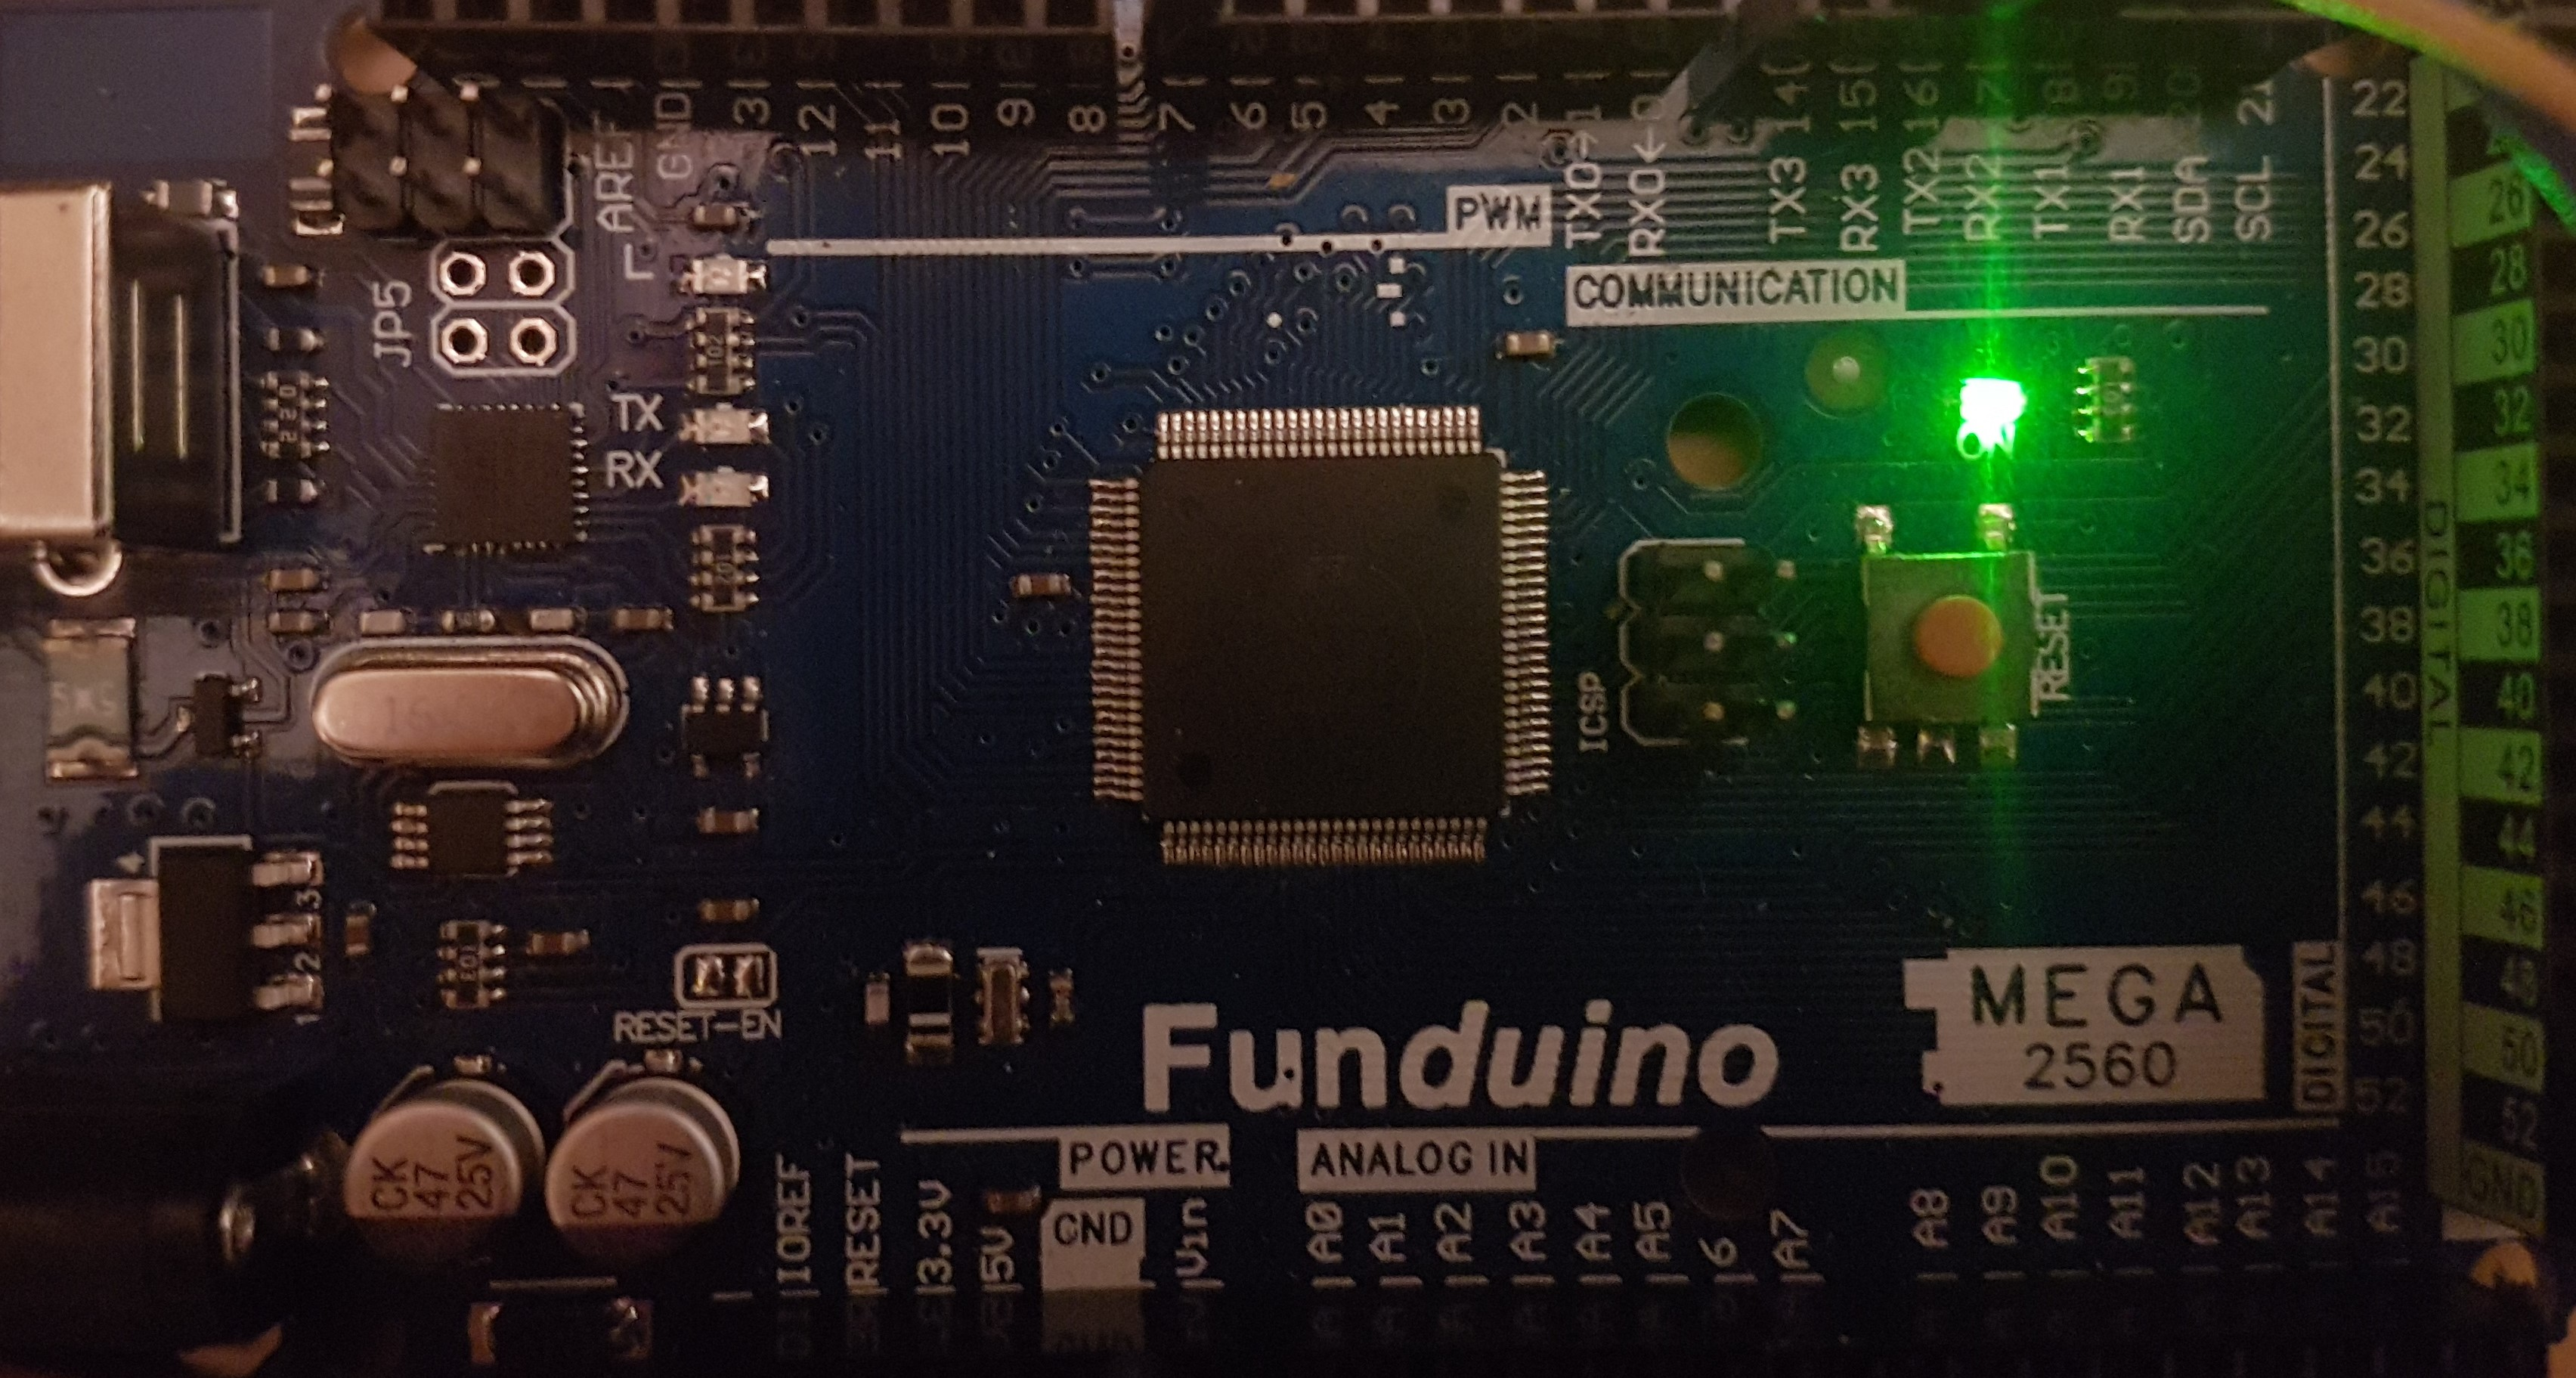
\includegraphics[width=0.48\textwidth]{graphics/Display_LED_OFF.jpg}}
\hfill
\caption{}
\label{fig:Hardware_LED_1}
\end{figure}
\end{enumerate}

\subsubsection{Programmablauf}\label{subsubsec:Hardware_Funktionstests_Programmablauf}

Der Test sieht wie folgt aus:

\begin{enumerate}
\item Bei Druck auf den Button des Displays
\begin{itemize}
\item Button-ID wird vom Display an den Mikrocontroller gesendet
\end{itemize}
\item Mikrocontroller verarbeitet die ID und löst bei \textbf{0x07 0x01 0xFF 0xFF 0xFF} folgende Funktionen aus:
\begin{itemize}
\item Unterhaltungstext schreiben.
\item Seite wechseln ``Getränk fertig``
\item Seite wechseln ``Cocktailliste``
\end{itemize}
\end{enumerate}

\subsubsection{Erwartung}\label{subsubsec:Hardware_Gesamtsystem_Erwartung2}

Wird der Menu-Button 0x01 auf der Seite 0x07 gedrückt, wird erwartet, dass der Mikrocontroller die Funktionen in folgender Reihenfolge abhandelt. 

\begin{enumerate}
%\item Statusübermittlung
%\begin{itemize}
%\item UART\_0-Schnittstelle muss angesprochen werden.
%\item Vor jedem Ausführen einer Funktion teilt der Mikrocontroller dem Computer mit, an welchem Punkt der Software er sich gerade befindet.
%\end{itemize}
\item Jeweilige Seite ändern (alle Seiten)
\begin{itemize}
\item UART\_1-Schnittstelle muss angesprochen werden.
\item Timer auf Seite ``Cocktail wird zubereitet`` betreibt eine Progressbar.
\item Jeweilige Seite wird aufgerufen.
\end{itemize}
\end{enumerate}
\newpage

\subsubsection{Ergebnis}\label{subsubsec:Hardware_Gesamtsystem_Ergebnis2}
\begin{enumerate}
%\item Statusübermittlung\\
%\\
%Wurde schon in \ref{subsubsec:Hardware_Gesamtsystem_Ergebnis} verifiziert.
%\\
%\begin{figure}[h!]
%	\centering	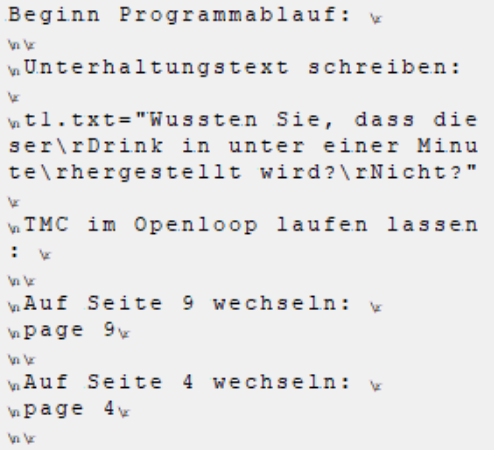
\includegraphics[width=0.4\textwidth]{graphics/Test_UART0_1.png}
%	\caption{Ausgabe der abzuhandelnden Schritte, wie sie gemäss Button 0xB1 der Seite 0x07 programmiert wurden, an die USB-Schnittstelle.} 
%	\label{fig:Hardware_Uart_0_1}
%\end{figure}\mbox{}\\

\item Gewünschte Seiten aufrufen\\
\\
Die Seiten werden wie im Programmfluss vorgegeben aufgerufen. Auch die Progressbar läuft wie erwartet von 0\% nach 100\%. Nach Ablauf des Programms sind weitere Eingaben möglich, die Software hängt sich während dem Betrieb also nicht auf. Die Erwartungen sind folglich verifiziert.
\begin{figure}[h!]
\centering
\subcaptionbox{Angezeigtes Display, während ein Cocktail zubereitet wird.\label{fig:Hardware_Anzeige_Zubereitung}}{	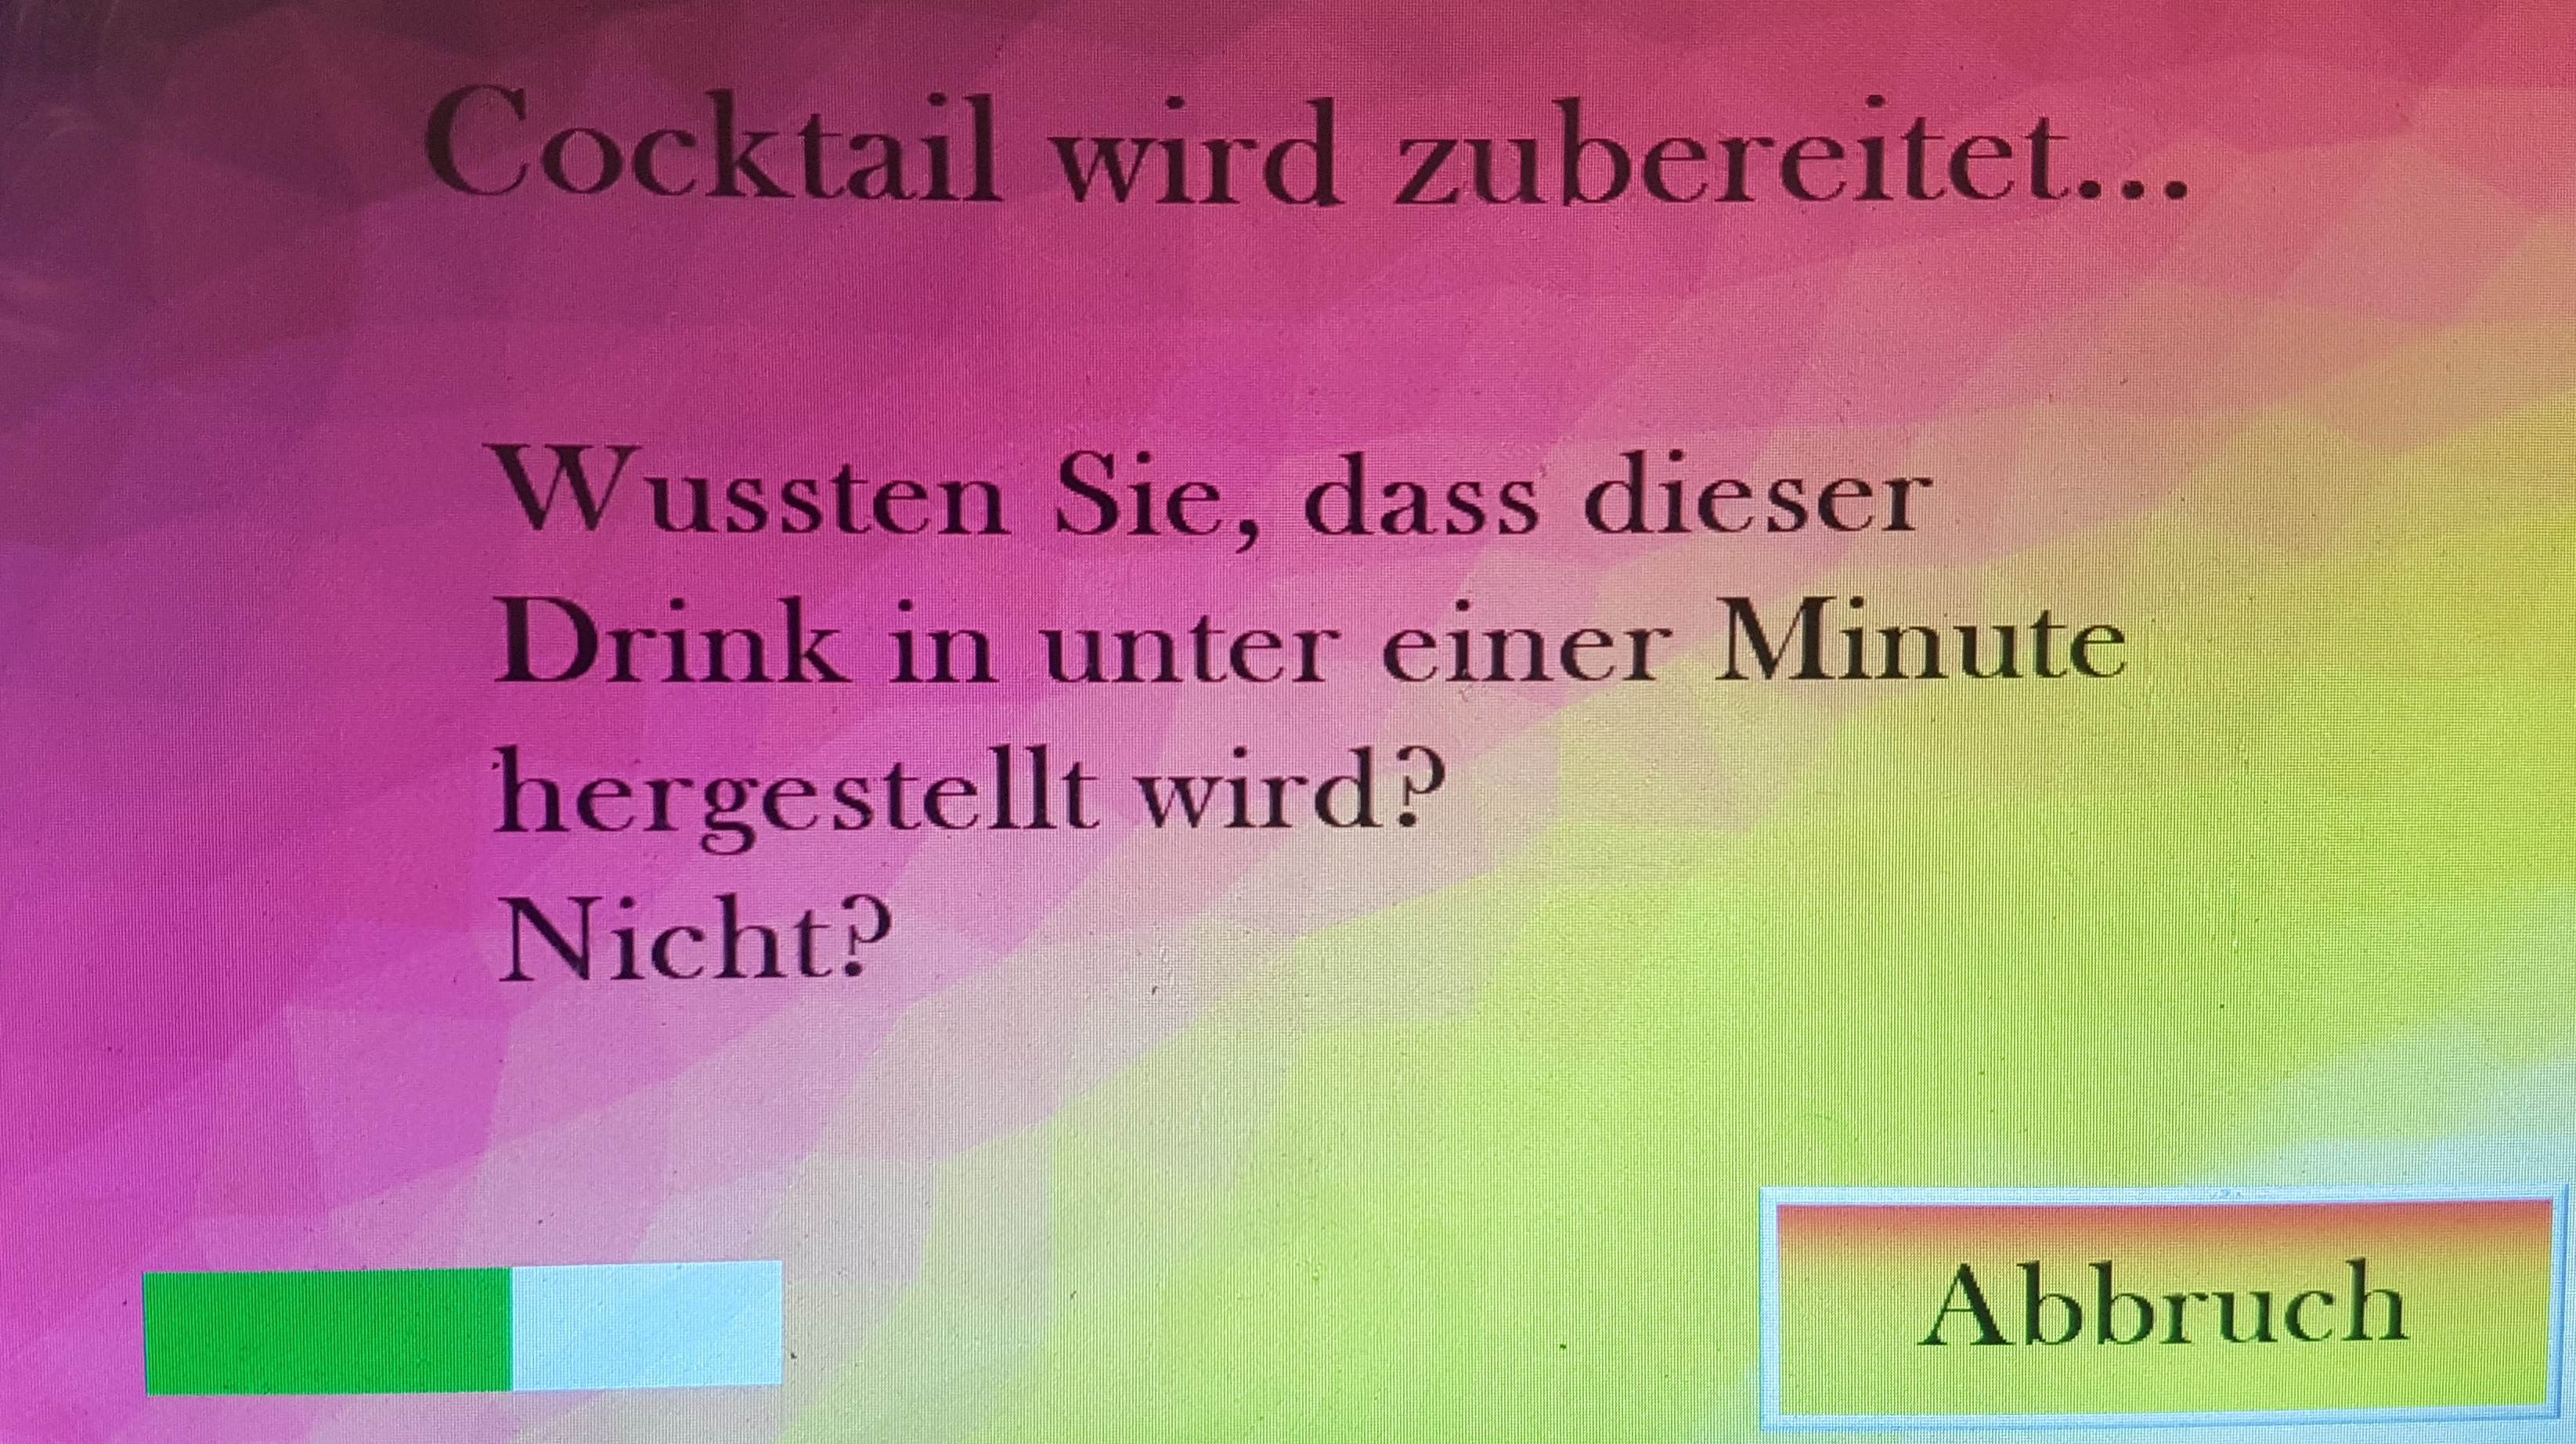
\includegraphics[width=0.48\textwidth]{graphics/Display_Cocktail_wird_zubereitet.jpg}}
\hfill
\subcaptionbox{Angezeigte Seite, wenn ein Getränk bereitsteht getrunken zu werden.\label{fig:Hardware_Getr_fertig}}{	
\includegraphics[width=0.48\textwidth]{graphics/Display_Getraenk_fertig.jpg}}
\hfill
\caption{Anzeigen des Displays}
\label{fig:Hardware_LED_1}
\end{figure}

\begin{figure}[h!]
	\centering	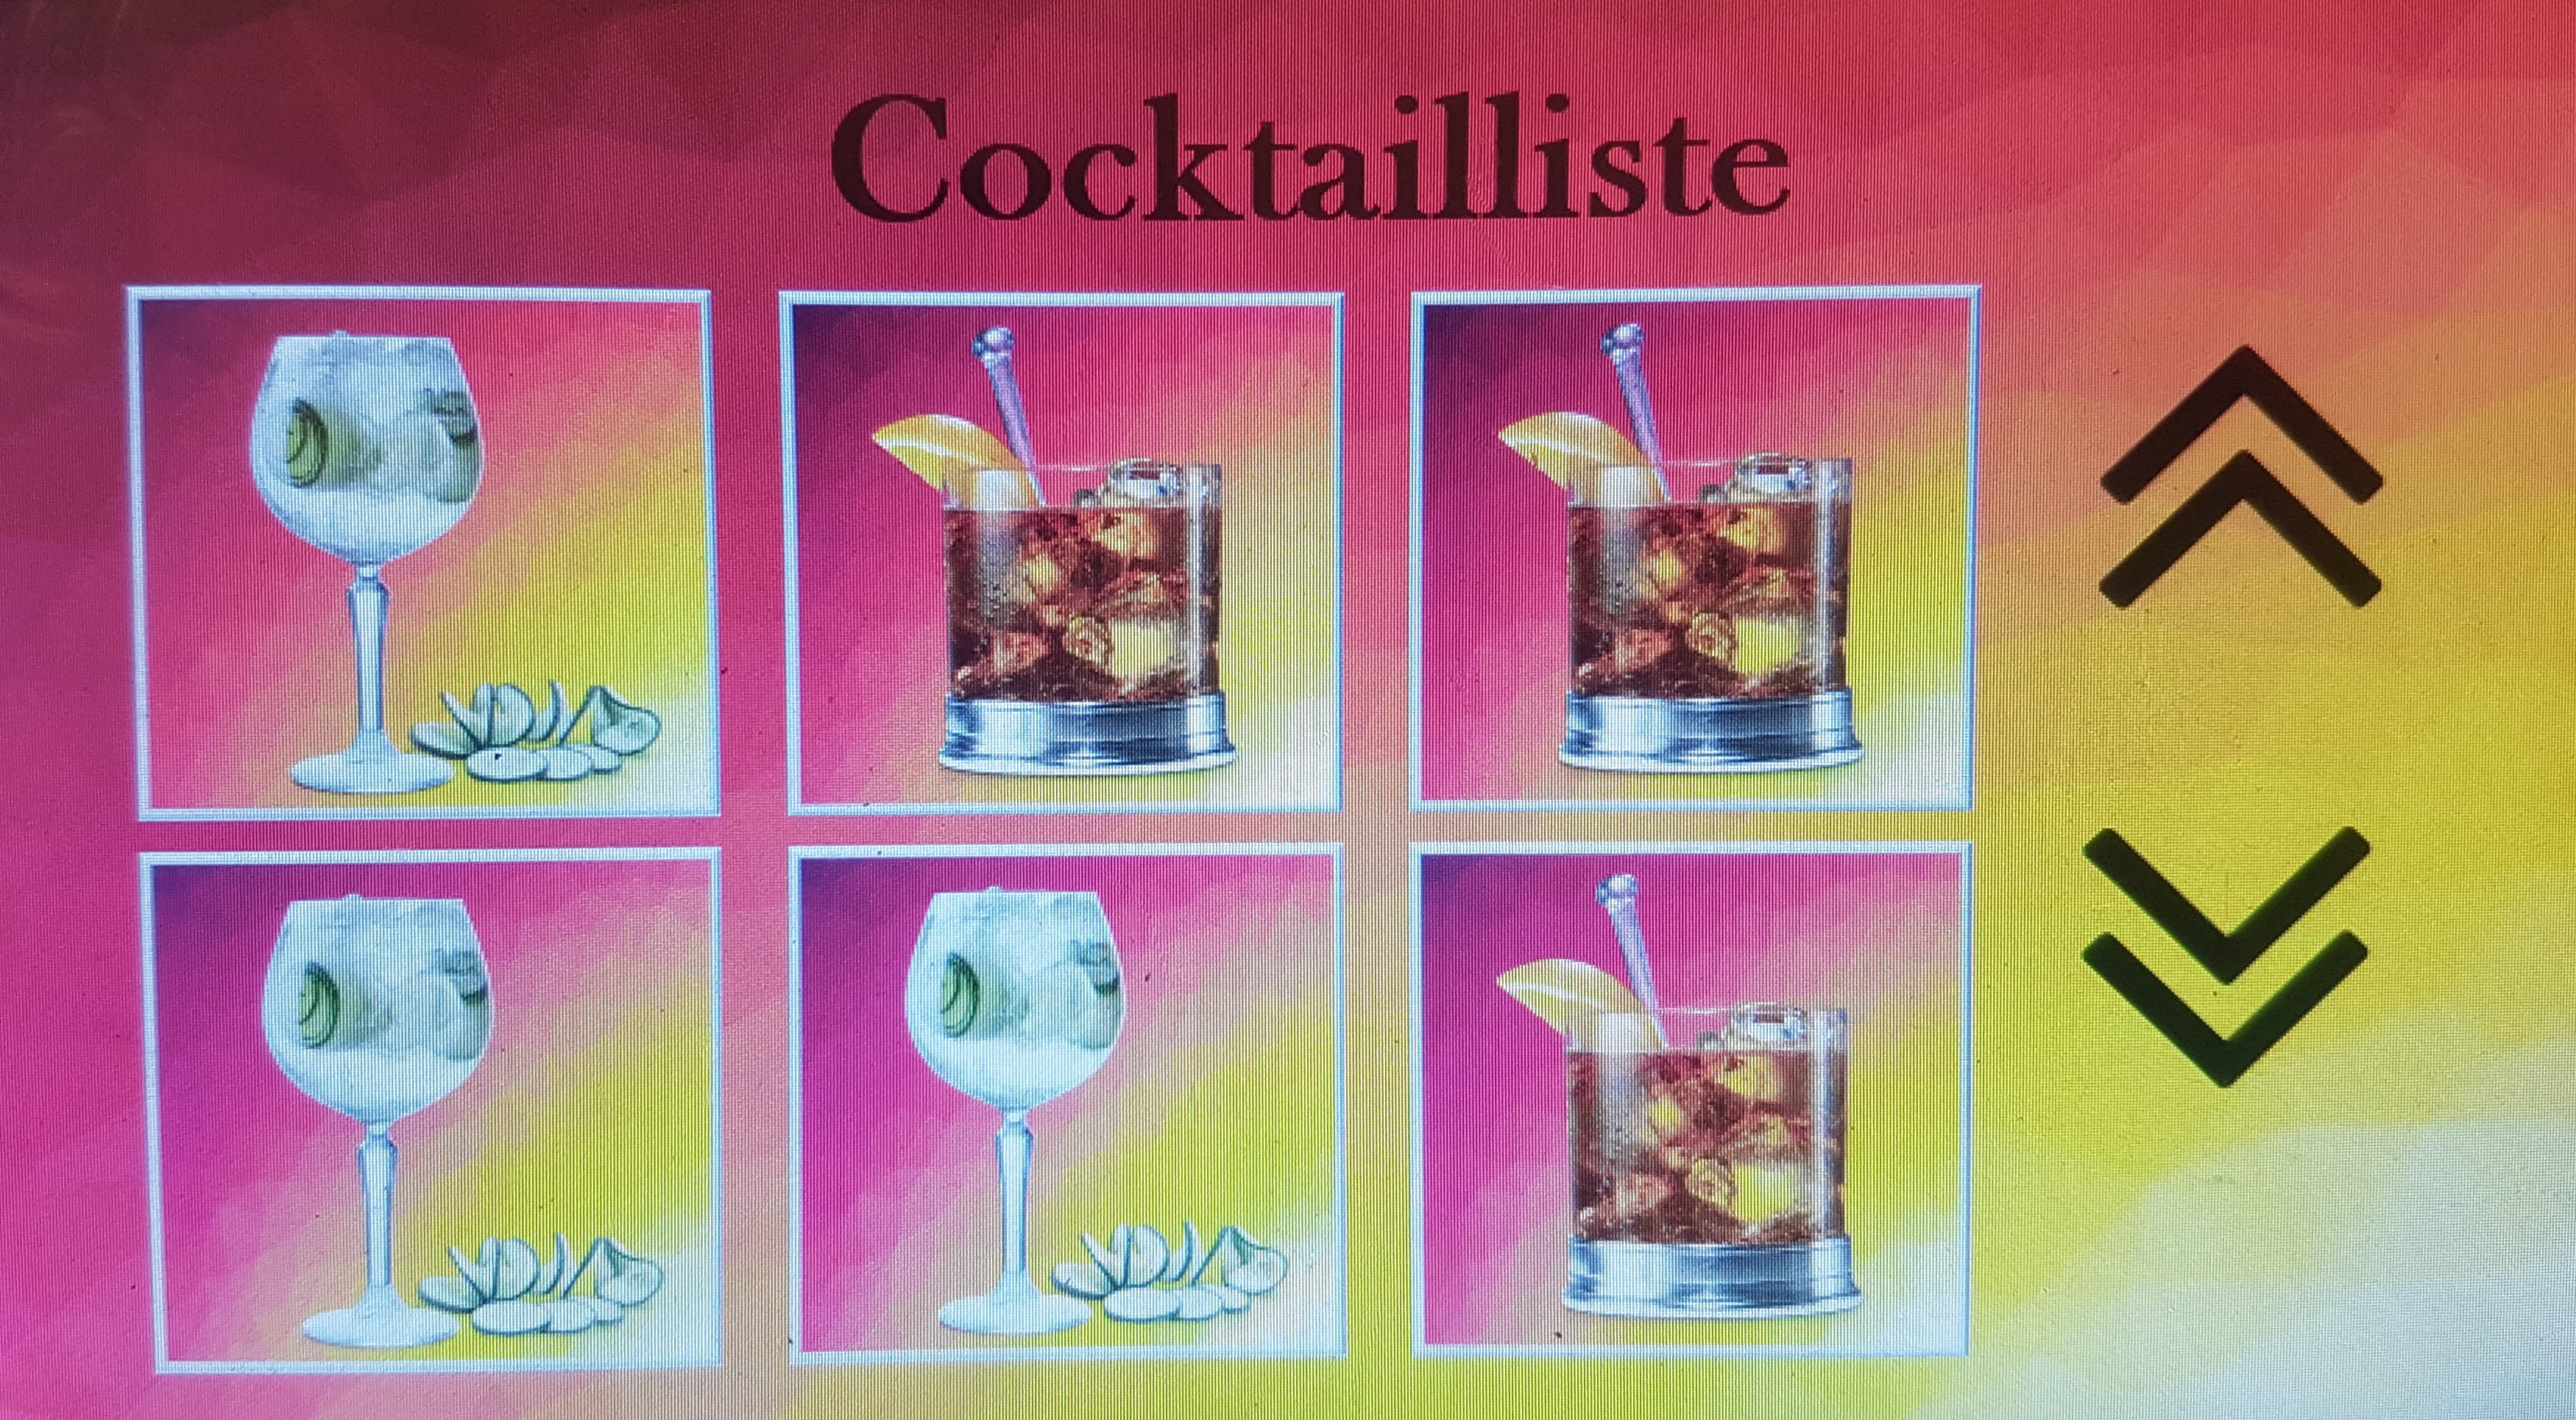
\includegraphics[width=0.6\textwidth]{graphics/Display_Cocktailliste.jpg}
	\caption{Angezeigtes Display, um Programm weiter bedienen zu können.} 
	\label{fig:Hardware_Cocktailliste}
\end{figure}
\end{enumerate}